\documentclass{beamer}
\mode<presentation>{
  \usetheme{Boadilla}
  \usefonttheme[onlylarge]{structurebold}
  \usefonttheme[stillsansseriflarge]{serif}
  \setbeamerfont*{frametitle}{size=\normalsize,series=\bfseries}
  % \setbeamertemplate{navigation symbols}{}
  \setbeamercovered{transparent}
}
\usepackage[english]{babel}
\usepackage[latin1]{inputenc}
\usepackage{times}
\usepackage[T1]{fontenc}
\usepackage{amsmath}
\usepackage{amssymb}
\usepackage{esint}
\usepackage{hyperref}
\usepackage{tikz}
\usepackage{xkeyval}
\usepackage{xargs}
\usepackage{xcolor}
\usepackage{verbatim}
\usepackage{listings}
\usepackage{multimedia}
\usepackage{bm}
\usepackage{siunitx}
\usetikzlibrary{
  arrows,
  calc,
  decorations.pathmorphing,
  decorations.pathreplacing,
  decorations.markings,
  fadings,
  positioning,
  shapes,
  arrows.meta
}
\usepgfmodule{oo}

\pgfdeclareradialshading{glow2}{\pgfpoint{0cm}{0cm}}{
  color(0mm)=(white);
  color(2mm)=(white);
  color(8mm)=(black);
  color(10mm)=(black)
}
\pgfdeclareradialshading{glow}{\pgfpoint{0cm}{0cm}}{
  color(0mm)=(white);
  color(5mm)=(white);
  color(9mm)=(black);
  color(10mm)=(black)
}

\begin{tikzfadingfrompicture}[name=glow fading]
  \shade [shading=glow] (0,0) circle (1);
\end{tikzfadingfrompicture}

\begin{tikzfadingfrompicture}[name=glow2 fading]
  \shade [shading=glow2] (0,0) circle (1);
\end{tikzfadingfrompicture}

\mode<handout>{
  \usepackage{pgfpages}
  \pgfpagesuselayout{4 on 1}[a4paper,landscape,border shrink=5mm]
  \setbeamercolor{background canvas}{bg=black!10}
}

\newcommand\pgfmathsinandcos[3]{%
  \pgfmathsetmacro#1{sin(#3)}%
  \pgfmathsetmacro#2{cos(#3)}%
}
\newcommand\LongitudePlane[3][current plane]{%
  \pgfmathsinandcos\sinEl\cosEl{#2} % elevation
  \pgfmathsinandcos\sint\cost{#3} % azimuth
  \tikzset{#1/.estyle={cm={\cost,\sint*\sinEl,0,\cosEl,(0,0)}}}
}
\newcommand\LatitudePlane[3][current plane]{%
  \pgfmathsinandcos\sinEl\cosEl{#2} % elevation
  \pgfmathsinandcos\sint\cost{#3} % latitude
  \pgfmathsetmacro\yshift{\cosEl*\sint}
  \tikzset{#1/.estyle={cm={\cost,0,0,\cost*\sinEl,(0,\yshift)}}} %
}
\newcommand\DrawLongitudeCircle[2][1]{
  \LongitudePlane{\angEl}{#2}
  \tikzset{current plane/.prefix style={scale=#1}}
  % angle of "visibility"
  \pgfmathsetmacro\angVis{atan(sin(#2)*cos(\angEl)/sin(\angEl))} %
  \draw[current plane] (\angVis:1) arc (\angVis:\angVis+180:1);
  \draw[current plane,dashed] (\angVis-180:1) arc (\angVis-180:\angVis:1);
}
\newcommand\DrawLatitudeCircleArrow[2][1]{
  \LatitudePlane{\angEl}{#2}
  \tikzset{current plane/.prefix style={scale=#1}}
  \pgfmathsetmacro\sinVis{sin(#2)/cos(#2)*sin(\angEl)/cos(\angEl)}
  % angle of "visibility"
  \pgfmathsetmacro\angVis{asin(min(1,max(\sinVis,-1)))}
  \draw[current plane,decoration={markings, mark=at position 0.6 with {\arrow{<}}},postaction={decorate},line width=.6mm] (\angVis:1) arc (\angVis:-\angVis-180:1);
  \draw[current plane,dashed,line width=.6mm] (180-\angVis:1) arc (180-\angVis:\angVis:1);
}
\newcommand\DrawLatitudeCircle[2][1]{
  \LatitudePlane{\angEl}{#2}
  \tikzset{current plane/.prefix style={scale=#1}}
  \pgfmathsetmacro\sinVis{sin(#2)/cos(#2)*sin(\angEl)/cos(\angEl)}
  % angle of "visibility"
  \pgfmathsetmacro\angVis{asin(min(1,max(\sinVis,-1)))}
  \draw[current plane] (\angVis:1) arc (\angVis:-\angVis-180:1);
  \draw[current plane,dashed] (180-\angVis:1) arc (180-\angVis:\angVis:1);
}
\newcommand\coil[1]{
  {\rh * cos(\t * pi r)}, {\apart * (2 * #1 + \t) + \rv * sin(\t * pi r)}
}
\makeatletter
\define@key{DrawFromCenter}{style}[{->}]{
  \tikzset{DrawFromCenterPlane/.style={#1}}
}
\define@key{DrawFromCenter}{r}[1]{
  \def\@R{#1}
}
\define@key{DrawFromCenter}{center}[(0, 0)]{
  \def\@Center{#1}
}
\define@key{DrawFromCenter}{theta}[0]{
  \def\@Theta{#1}
}
\define@key{DrawFromCenter}{phi}[0]{
  \def\@Phi{#1}
}
\presetkeys{DrawFromCenter}{style, r, center, theta, phi}{}
\newcommand*\DrawFromCenter[1][]{
  \setkeys{DrawFromCenter}{#1}{
    \pgfmathsinandcos\sint\cost{\@Theta}
    \pgfmathsinandcos\sinp\cosp{\@Phi}
    \pgfmathsinandcos\sinA\cosA{\angEl}
    \pgfmathsetmacro\DX{\@R*\cost*\cosp}
    \pgfmathsetmacro\DY{\@R*(\cost*\sinp*\sinA+\sint*\cosA)}
    \draw[DrawFromCenterPlane] \@Center -- ++(\DX, \DY);
  }
}
\newcommand*\DrawFromCenterText[2][]{
  \setkeys{DrawFromCenter}{#1}{
    \pgfmathsinandcos\sint\cost{\@Theta}
    \pgfmathsinandcos\sinp\cosp{\@Phi}
    \pgfmathsinandcos\sinA\cosA{\angEl}
    \pgfmathsetmacro\DX{\@R*\cost*\cosp}
    \pgfmathsetmacro\DY{\@R*(\cost*\sinp*\sinA+\sint*\cosA)}
    \draw[DrawFromCenterPlane] \@Center -- ++(\DX, \DY) node {#2};
  }
}
\makeatother

% not mandatory, but I though it was better to set it blank
\setbeamertemplate{headline}{}
\def\beamer@entrycode{\vspace{-\headheight}}

\tikzstyle{snakearrow} = [decorate, decoration={pre length=0.2cm,
  post length=0.2cm, snake, amplitude=.4mm,
  segment length=2mm},thick, ->]

%% document-wide tikz options and styles

\tikzset{%
  % >=latex, % option for nice arrows
  inner sep=0pt,%
  outer sep=2pt,%
  mark coordinate/.style={inner sep=0pt,outer sep=0pt,minimum size=3pt,
    fill=black,circle}%
}
\tikzset{
  % Define standard arrow tip
  >=stealth',
  % Define style for boxes
  punkt/.style={
    rectangle,
    rounded corners,
    draw=black, very thick,
    text width=8em,
    minimum height=2.5em,
    text centered},
}

\tikzset{onslide/.code args={<#1>#2}{%
    \only<#1>{\pgfkeysalso{#2}}
    % \pgfkeysalso doesn't change the path
  }}
\tikzset{alt/.code args={<#1>#2#3}{%
    \alt<#1>{\pgfkeysalso{#2}}{\pgfkeysalso{#3}}
    % \pgfkeysalso doesn't change the path
  }}
\tikzset{temporal/.code args={<#1>#2#3#4}{%
    \temporal<#1>{\pgfkeysalso{#2}}{\pgfkeysalso{#3}}{\pgfkeysalso{#4}}
    % \pgfkeysalso doesn't change the path
  }}

\makeatletter
\newbox\@backgroundblock
\newenvironment{backgroundblock}[2]{%
  \global\setbox\@backgroundblock=\vbox\bgroup%
  \unvbox\@backgroundblock%
  \vbox to0pt\bgroup\vskip#2\hbox to0pt\bgroup\hskip#1\relax%
}{\egroup\egroup\egroup}
\addtobeamertemplate{background}{\box\@backgroundblock}{}
\makeatother

\title{Building Single Molecules from Single Atoms}
\date{Sep 5, 2019}
\author[Yichao Yu]{Yichao Yu\\
  \vspace{0.5cm}
  {\footnotesize Lee Liu, Kenneth Wang, Lewis Picard, Jonathan Hood}\\
  {\footnotesize Jessie T. Zhang, Eliot Fenton, Yen-Wei Lin}}
\institute{Ni Group/Harvard}

\begin{document}

\pgfdeclarelayer{tweezer}
\pgfsetlayers{tweezer,main}
\pgfooclass{tweezer}{
  \method tweezer() {
  }
  \method drawTweezer(#1,#2,#3) {
    \begin{pgfonlayer}{tweezer}
      \shade[shading=radial,path fading=glow fading,shift={(#1,#2)},rotate=90,yscale=1,
      fill opacity=0.9,inner color=#3]
      plot[draw,samples=200,domain=-1.5:1.5] function {sqrt(0.01 + x**2 / 5)}
      -- plot[draw,samples=200,domain=1.5:-1.5] function {-sqrt(0.01 + x**2 / 5)};
    \end{pgfonlayer}
  }
  \method drawAtom(#1,#2,#3,#4) {
    \fill [#4,path fading=glow2 fading] (#1,#2) circle (#3);
  }
  \method drawNaAtom(#1,#2,#3) {
    \pgfoothis.drawAtom(#1,#2,#3,orange);
  }
  \method drawCsAtom(#1,#2,#3) {
    \pgfoothis.drawAtom(#1,#2,#3,blue);
  }
  \method drawNaTweezer(#1,#2) {
    \pgfoothis.drawTweezer(#1,#2,orange!35!black!30);
  }
  \method drawCsTweezer(#1,#2) {
    \pgfoothis.drawTweezer(#1,#2,blue!30!black!30);
  }
  \method up(#1,#2) {
    \pgfoothis.drawCsTweezer(#1,#2);
    \pgfoothis.drawNaAtom(#1,#2+0.06,0.12);
    \pgfoothis.drawCsAtom(#1,#2-0.06,0.16);
  }
  \method down(#1,#2) {
    \pgfoothis.drawCsTweezer(#1,#2);
    \pgfoothis.drawCsAtom(#1,#2+0.06,0.16);
    \pgfoothis.drawNaAtom(#1,#2-0.06,0.12);
  }
  \method naTrap(#1,#2) {
    \pgfoothis.drawNaTweezer(#1,#2);
    \pgfoothis.drawNaAtom(#1,#2,0.12);
  }
  \method csTrap(#1,#2) {
    \pgfoothis.drawCsTweezer(#1,#2);
    \pgfoothis.drawCsAtom(#1,#2,0.16);
  }
}
\pgfoonew \mytweezer=new tweezer()

{
  \usebackgroundtemplate{
    \makebox[\paperwidth][c]{\centering\includegraphics[width=\paperwidth]{front_bg.png}}
  }
  \setbeamercolor{title}{fg=white}
  \setbeamercolor{author}{fg=white}
  \setbeamercolor{institute}{fg=white}
  \setbeamercolor{date}{fg=white}
  \begin{frame}{}
    \titlepage
  \end{frame}
}

% I'm going to talk about our experiment on ....
% I was told that not everyone here is familar with molecules
% so I'll start with what we are doing and why we are using .....

% (1min)

% Most of you are probably familar with atoms
% * Laser cooling/trapping
% * Internal state control
% * High fidelity imagining
% * ... (and you can put in your favorate property of atoms here)
% There are way too many examples for this so here's just one result from
% Greiner group that demonstrates all the properties I mentioned.

% On the other hand, there's basically one problem with atoms
% * Too simple
% Weak interaction so need to try very hard to make a non-trivial system
% Few internal states so that the tricks that you can play with them is limited.

% (3min)

% Molecule
% * Interaction
% * Rich internal structure (more for polyatomic molecules)
% If we can have the same control

% Applications
% * Quantum information
% * Quantum simulations
% * Quantum chemistry
% * Precision measurement

% Spoiler: we cant achieve the same level of control yet
% That's what I'll talk about

% (5min)

\begin{frame}[t]{From Atom to Molecule}
  \begin{center}
    \begin{tikzpicture}
      \node at (-3, 0) {\LARGE Atom};
      \node[align=left, text width=6cm, below] at (-3, -0.5) {
        \begin{itemize}
        \item Laser cooling/trapping
        \item Internal state control
        \item High fidelity imagining\\
          \visible<1-3>{$\vdots$}
        \end{itemize}
      };
      \visible<2-3>{
        \node[below,align=center] at (-3, -3.5)
        {\includegraphics[width=4cm]{lithium_microscope}\\
          {\tiny Nature 545, 462-466 (2017)}};
      }
      \visible<3->{
        \node at (3, 0) {\LARGE Molecule};
        \node[align=left, text width=6cm, below] at (3, -0.5) {
          \begin{itemize}
          \item Strong interaction
          \item Rich internal structure
          \end{itemize}
        };
      }
      \visible<4>{
        \node[align=center] at (-4.6, -5.5) {
          \usebeamercolor[fg]{frametitle}{\small Quantum Chemistry}\\
          \includegraphics[width=2.3cm]{quantum_chemistry}\\
          {\tiny Nature 464, 1324 (2010)}};
        \node[align=center] at (-1.5, -4.5) {
          \usebeamercolor[fg]{frametitle}{\small Quantum Simulation}\\
          \includegraphics[width=2.9cm]{quantum_simulation}\\
          {\tiny Nat. Phys. 2, 341 (2006)}};
        \node[align=center] at (3.6, -3.4) {
          \usebeamercolor[fg]{frametitle}{\small Quantum Computing}\\
          \includegraphics[width=2.9cm]{quantum_computing}\\
          {\tiny Phys. Rev. Lett. 97, 33003 (2006)}};
        \node[align=center] at (2.8, -6.35) {
          \usebeamercolor[fg]{frametitle}{\small Precision Measurement}\\
          \includegraphics[width=3.6cm]{edm}\\
          {\tiny Science 343, p. 269-272 (2014)}};
      }
    \end{tikzpicture}
  \end{center}
\end{frame}

% As I said, cooling or in general controlling molecules is hard.
% There has been a few ways that people used to obtain ultracold molecules:
% * Direct cooling
% -- Hard because absense of cycling transition.
% -- But can be done on some molecules that sort of do.
% -- Pioneered by ... including here at Harvard in the Doyle group.
% * Making molecules from atoms
% -- Take advantage of atom cooling.
% -- Use a combination of magnetic and optical transitions.
% -- First realized by ....
% * Our approach
% -- Combine the bulk gas approach with recent progress on optical tweezers
% -- Do not rely as heavily on collisional properties for cooling and overlapping.
% -- Naturally single site resolution and manipulation
% -- Fast cycle time/high fidelity

% (8min)

\begin{frame}[t]{Path to Ultracold Molecules}
  \begin{center}
    \begin{tikzpicture}
      \visible<1-2> {
        \node[align=center,below] at (-3, 0) {\textbf{\large Direct molecule cooling}\\
          ``Diagonal molecules'':\\
          CaF, SrF, YO, $\dots$\\
          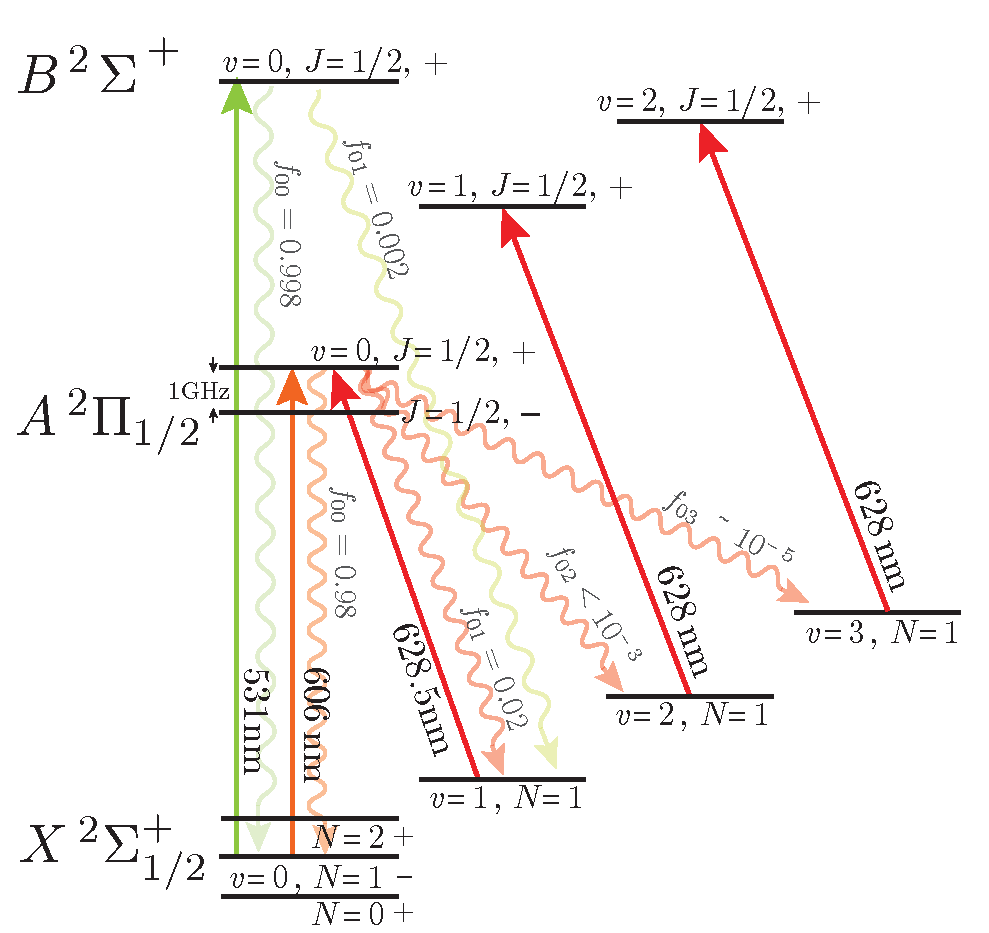
\includegraphics[width=5cm]{caf_levels}\\
          {\tiny Phys. Rev. Lett. 119, 103201 (2017)}
        };
      }
      \visible<2-> {
        \node[align=center,below,text width=6cm] at (3, 0)
        {\textbf{\large Making molecule from atoms}\\
          Bi-Alkali/Alkaline Earth:\\
          KRb, RbCs, NaK, LiNa, $\dots$\\
          \vspace{0.8cm}
          \begin{enumerate}
          \item Cold gas of atoms
          \item Feshbach association
          \item STIRAP
          \end{enumerate}
        };
      }
      \visible<3-> {
        \node[align=center,below,text width=6cm] at (-3, 0)
        {\textbf{\large Assemble molecule in tweezers}\\
          \vspace{0.4cm}
          \begin{enumerate}
          \item Atoms in tweezers
          \item Optical association
          \end{enumerate}
          \vspace{0.4cm}
          \visible<4-> {
            \begin{itemize}
            \item Single site detection
            \item Single site addressing
            \item Control loading and interaction
              by rearranging.
            \end{itemize}
          }
        };
        \node[right] at (-2.5, -6) {\includegraphics[width=6cm]{molecule_in_tweezers}};
      }
    \end{tikzpicture}
  \end{center}
\end{frame}

% So here's an outline for the rest of my talk.
% I'll first give an overview of out experiment, both the procedure and the apparatus
% Then I'll talk about a few intersting aspect of the atom part of our experiment
% i.e. some trapping and cooling issues that we've had
% which required us to develop new techniques for our setup.
% Finally, I'll talk about our progress on measuring the interaction between atoms
% and making molecules.
% (9min)
\begin{frame}{Outline}
  \tableofcontents
\end{frame}

\section{System Overview}

% As I said, in our experiment, we make molecules from atoms inside the optical tweezer
% so the obvious first step is to get the atoms in there.
% Load directly from the MOT and further cool in the tweezer which I'll talk about later.

% We load the Na and Cs atoms separately in two tweezers, that are ... apart.
% Obviously, serves no good to make molecules

% After merge without killing or heating the atoms
% Try to make molecules or do some study on the interaction to help us make molecules

\begin{frame}[t]{Steps}
  \vspace{-0.5cm}
  \begin{center}
    \begin{tikzpicture}[scale=0.75]
      \mytweezer.drawCsTweezer(0, 0)
      \mytweezer.drawNaTweezer(-1, 0)
      \mytweezer.drawCsAtom(-0.07, 0.08, 0.22)
      \mytweezer.drawNaAtom(-1.06, -0.09, 0.27)

      \mytweezer.drawCsTweezer(0, -3.1)
      \mytweezer.drawNaTweezer(-1, -3.1)
      \mytweezer.drawCsAtom(0.0, -3.1, 0.12)
      \mytweezer.drawNaAtom(-1.0, -3.1, 0.16)

      \mytweezer.drawCsTweezer(-1, -7.0)
      \mytweezer.drawNaAtom(-1.05, -6.87, 0.16)
      \mytweezer.drawCsAtom(-0.95, -7.13, 0.12)

      \visible<1-4> {
        \fill[white,temporal=<1>{opacity=0.82}{opacity=0}{opacity=0.5}]
        (-1.5, 1.5) rectangle (0.5, -1.5);
        \fill[white,temporal=<2>{opacity=0.82}{opacity=0}{opacity=0.5}]
        (-1.5, 1.5 - 3.1) rectangle (0.5, -1.5 - 3.1);
        \fill[white,temporal=<3-4>{opacity=0.82}{opacity=0}{opacity=0.5}]
        (-1.5, 1.5 - 7.0) rectangle (-0.5, -1.5 - 7.0);
      }

      \visible<2->{
        \begin{scope}[alt=<2>{opacity=0.7}{opacity=0.35}]
          \draw[orange,dotted,line width=1.2] (-1, -0.4) -- (-1, -2.9);
          \draw[blue,dotted,line width=1.2] (0, -0.15) -- (0, -2.9);
        \end{scope}
      }

      \visible<3->{
        \begin{scope}[alt=<3>{opacity=0.7}{opacity=0.35}]
          \draw[->,orange,line width=1.2] (-1, -3.3) -- (-1, -6.7);
          \draw[->,blue,domain=-3.3:-6.7,smooth,variable=\y,line width=1.2]
          plot ({atan((\y+4.7) * 5) / 170 - 0.5},{\y});
        \end{scope}
      }

      \node[right] at (1, 0) {\usebeamercolor[fg]{frametitle}{\large Loading}};
      \visible<2-> {
        \node[right] at (1, -3.1) {\usebeamercolor[fg]{frametitle}{\large Cooling}};
      }
      \visible<3-> {
        \node[right] at (1, -5.05) {\usebeamercolor[fg]{frametitle}{\large Merging}};
      }
      \visible<4-> {
        \node[right,align=left] at (1, -7)
        {\usebeamercolor[fg]{frametitle}{\large Interaction /}\\
          \usebeamercolor[fg]{frametitle}{\large Molecule}};
      }
      \visible<5-> {
        \node[align=center] at (8, -3.5) {\includegraphics[width=4cm]{science_cover}\\
          {\tiny Science 360 6391, 2018}};
      }
    \end{tikzpicture}
  \end{center}
\end{frame}

% The whole experiment looks like this
% And Na MOT
\begin{frame}{}
  \begin{center}
    \begin{tikzpicture}
      \node at (-3, 0) {\includegraphics[width=9cm]{chamber}};
      \visible<2-> {
        \draw[white, line width=2] (-4.5, -0.8) ellipse (0.25 and 0.4);
        \draw[white, line width=1.5] (-4.5, -0.4) -- (-0.5, 1.65);
        \draw[white, line width=1.5] (-4.5, -1.2) -- (-0.5, -1.65);
        \draw[white, line width=3] (-0.5, 1.65) rectangle (4.5, -1.65);
        \node at (2, 0) {\includegraphics[width=5cm]{na_mot}};
        \fill[black, opacity = 0.3, even odd rule]
        (-0.5, 1.65) rectangle (4.5, -1.65) (1.9, 0.35) circle (0.3);
        \node[below, white] at (1.9, -0.1) {\textbf{\small Na MOT}};
      }
    \end{tikzpicture}
  \end{center}
\end{frame}

% (12 min)

\section{Trapping and Cooling of Atoms}

% Our experiment starts with trapped atoms in tweezers.
% People have demonstrated before us.
% It sounds simple but turns out to be anything but.

% Well, Cs is fine.
% Got without too much effort.
% But Na is not.
% A few properties.
% * Low vapor pressure (fewer atoms to load from)
% * Broad linewidth (higher Doppler temperature)
% * Low mass (move faster and higher recoil velocity/energy)
% * Small HF structure (6 line width, worse PG cooling)

% Fine just need deeper trap but run into the real issue
% * Light shift
% In order to load, need cooling in the tweezer
% However, since we need such a deep trap, light shift turns off the cooling
% Got stuck in an awkward situation where a shallow trap can keep the cooling work but
% can't hold the atom while a deeper trap can hold the atom but the atom doesn't want to come in.

% Tried a bunch of ways (turn trap around atom, two wavelengths to cancel the trap)
% before Nick came up with a genius/crazy idea that people have used on large ODT.

% See laser cooling relies on scattering that happens at a rate of tens of MHz
% OTOH, the tweezer is only needed for trap motion that happens ~ few hundred kHz.
% Means that if we switch the tweezer on and off. .....

% Tried on Cs
% Essentially made a magic trap.

% Then tried on Na, it worked.
% Na live atom.

% Na and Cs 60 % loading on a good day.
% (20min)
\begin{frame}{Single Atom in Tweezer}
  \begin{columns}[t]
    \column{5cm}
    \begin{block}{}
      \begin{itemize}
      \item Previously done with Rb
      \item<2-> Works for Cs
      \item<3-> Doesn't work for Na
      \end{itemize}
    \end{block}
    \column{6cm}
    \begin{center}
      \begin{tikzpicture}
        \visible<2> {
          \node at (0, 0)
          {\includegraphics[width=6cm]{cs-histogram}};
        }
        \visible<3> {
          \node at (0, 0)
          {\includegraphics[width=5cm]{na-noatom}};
        }
        \visible<4> {
          \node[text width=6cm] at (0, 0) {
            \begin{block}{Issues with Na}
              \begin{itemize}
              \item Low vapor pressure
              \item Broad linewidth
              \item Low mass
              \item Small hyperfine structure
              \end{itemize}
            \end{block}
          };
        }
      \end{tikzpicture}
    \end{center}
  \end{columns}
\end{frame}

\begin{frame}{Real Issue with Na: Light Shift}
  \vspace{-1cm}
  \begin{columns}
    \column{5.7cm}
    \begin{center}
      \only<-3>{\includegraphics[width=5.5cm]{light-shift.png}}
      \only<4->{
        \begin{block}{Trap modulation}
          Alternate between trap and resonant {\small (cooling and imaging)} light
          at $2.5$\ MHz\\
          {\small $f_{trap}=100\sim500$\ kHz}\\
          {\small $\Gamma=2\pi\times 10$\ MHz}
        \end{block}
        \includegraphics[width=5cm]{switching.png}
      }
    \end{center}
    \column{5.8cm}
    \begin{center}
      \begin{tikzpicture}
        \visible<2-4>{
          \node[align=center] at (0, 0) {Cs single atom imaging\\
            \includegraphics[width=5.5cm]{det-vs-photon-dc}};
        }
        \visible<3-5>{
          \node[align=center, text width=5cm] at (0, -4.5) {
            \begin{block}{}
              \begin{itemize}
              \item Low imaging signal
              \item No cooling in tweezer
              \end{itemize}
            \end{block}
          };
        }
        \visible<5->{
          \node[align=center] at (0, 0) {Cs single atom imaging\\
            \includegraphics[width=5.5cm]{det-vs-photon-ac}};
        }
        \visible<6->{
          \node at (0, -4.5)
          {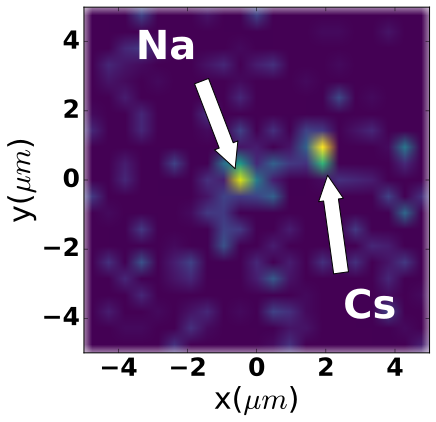
\includegraphics[width=4cm]{../../experiments/nacs_atoms/imgs/single_viridis.png}};
        }
      \end{tikzpicture}
    \end{center}
  \end{columns}
\end{frame}

% Since we want to control the state of the molecule by controlling the state of the atom
% including the motional state,
% we want to cool the atoms in the trap to the motional ground state in the tweezer.

% We use RSC

% Again, this has been done in other tweezers/optical lattice for some species.
% And you can probably guess which atom is harder.
\begin{frame}{Raman Sideband Cooling}
  \vspace{-0.5cm}
  \begin{tikzpicture}
    \visible<-4> {
      \node at (-3, 0) {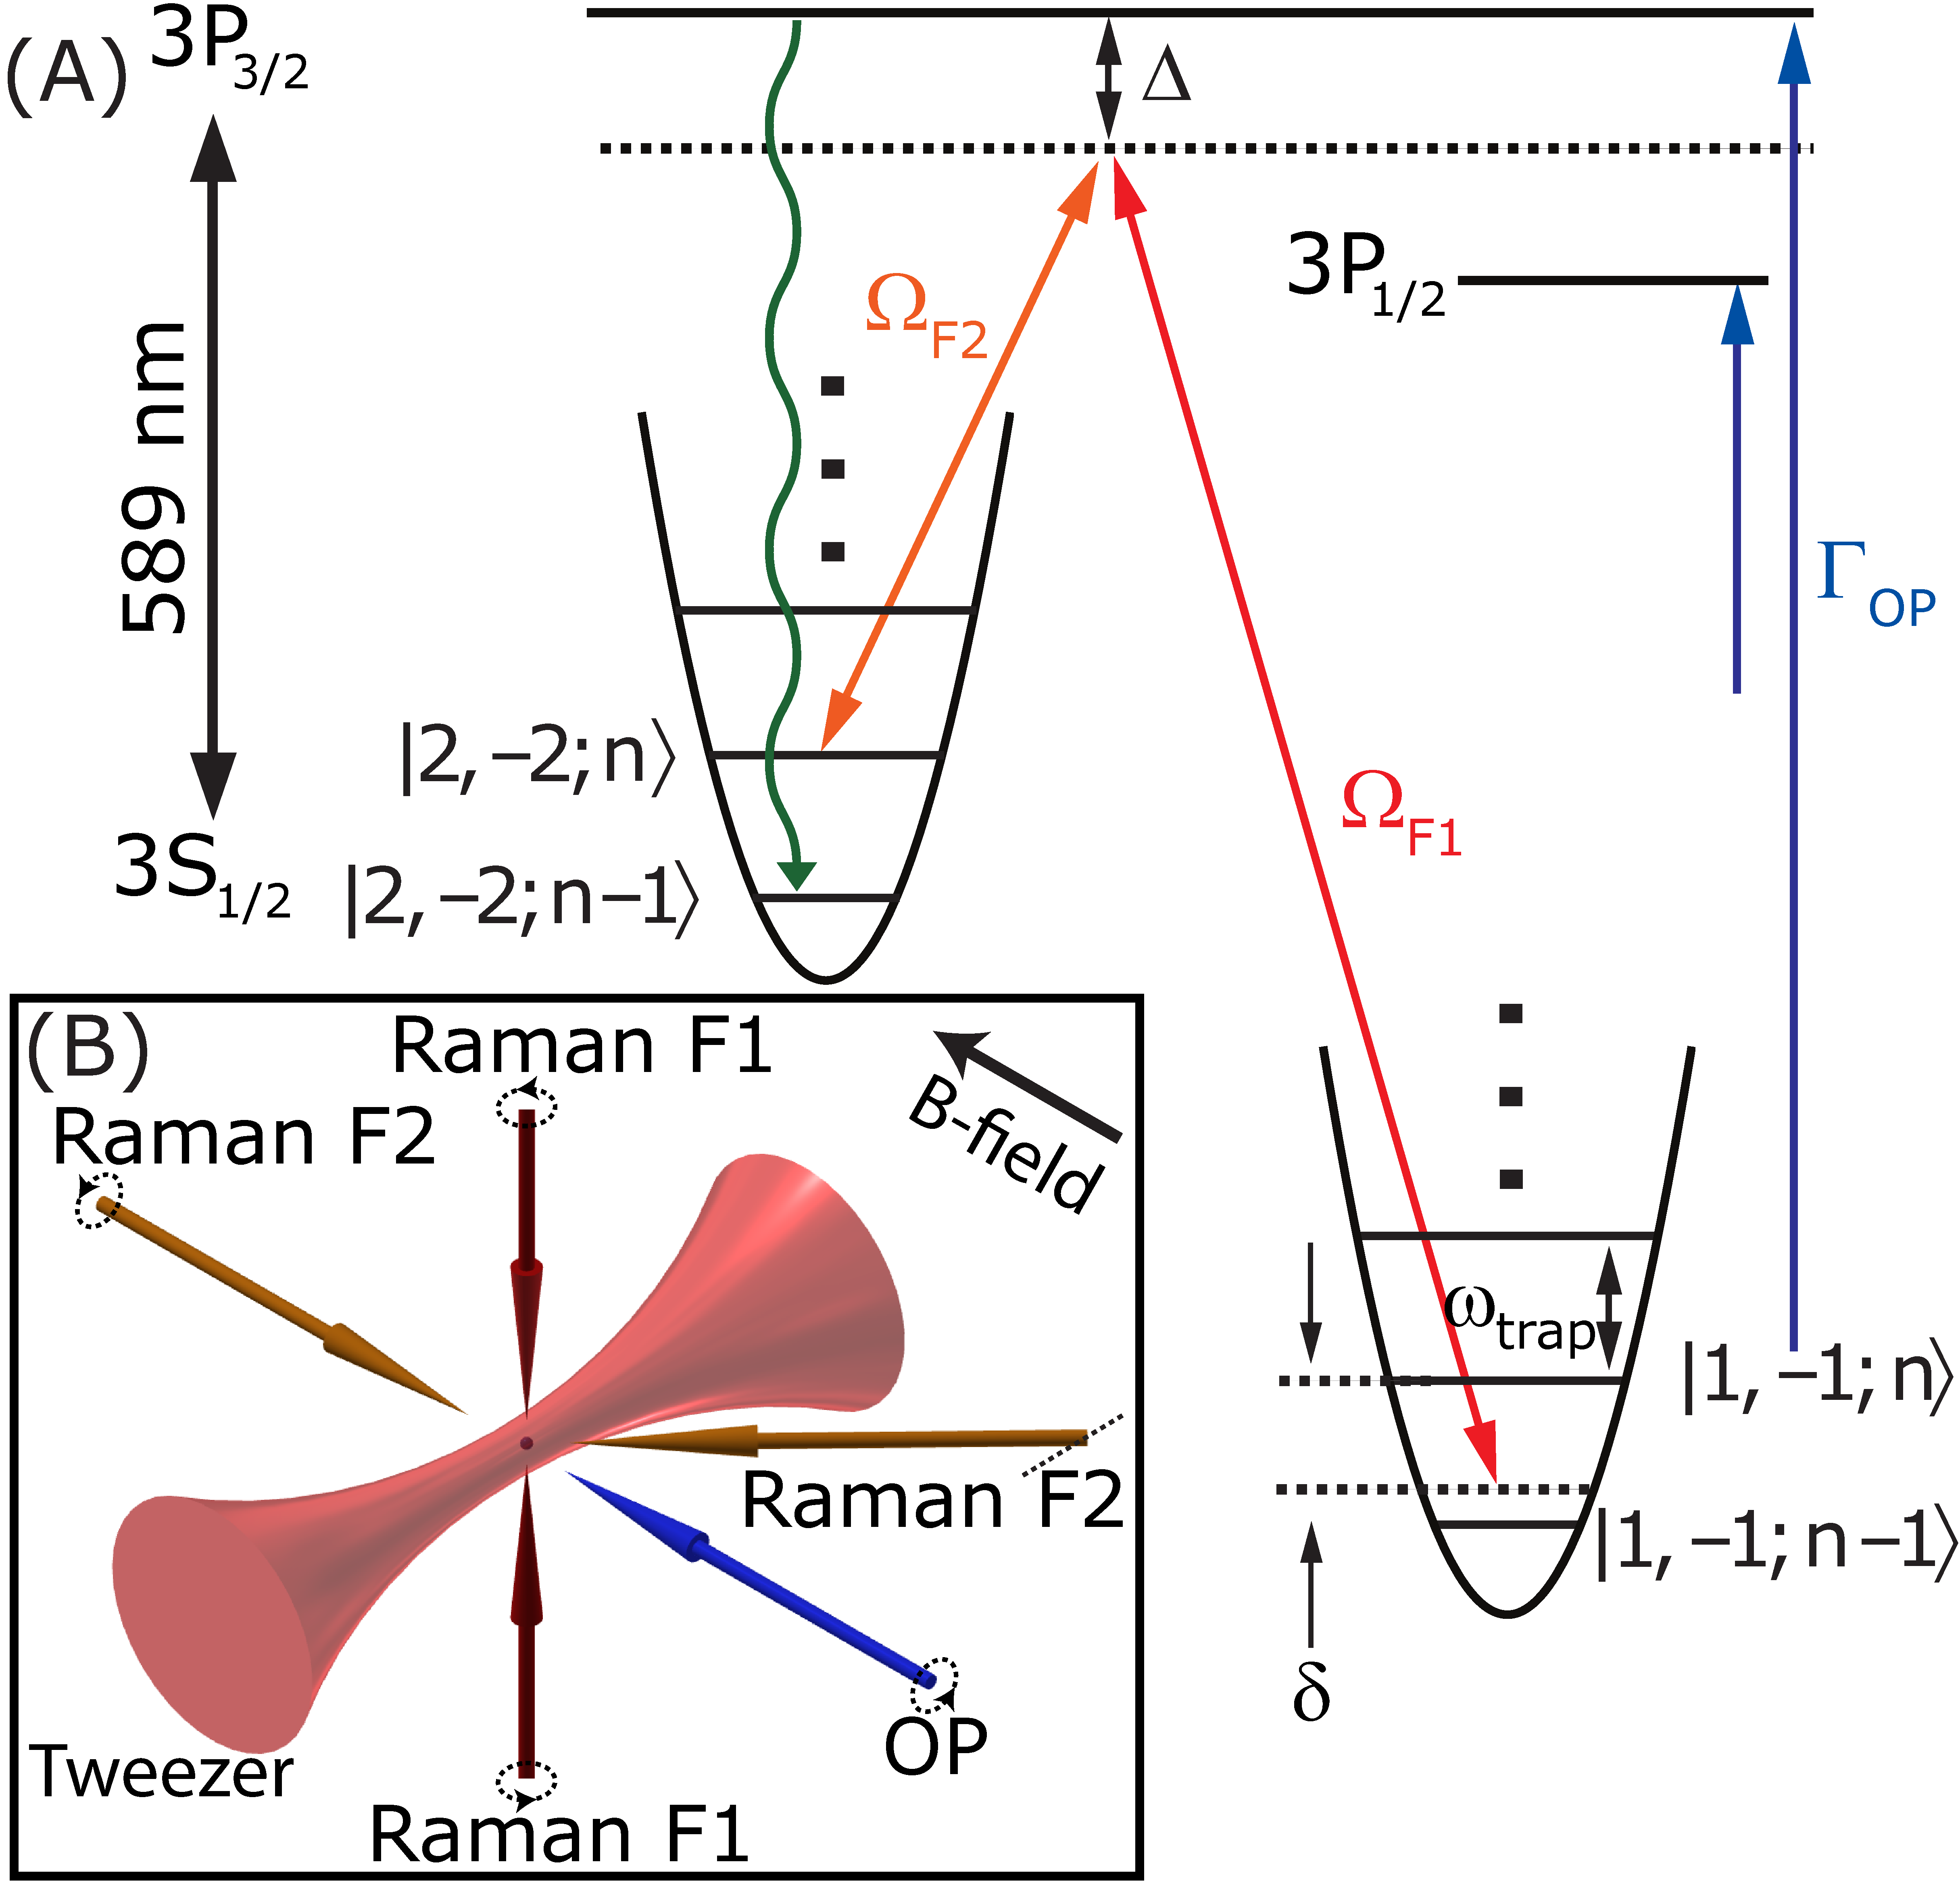
\includegraphics[width=5.5cm]{Na_RSC_schematic}};
    }
    \visible<2-> {
      \node[text width=5.5cm] at (3, 2) {
        \begin{block}{Large Lamb Dicke parameter}
          \begin{itemize}
          \item<3-> Large recoil heating
          \item<4-> Many sideband orders
          \item<5-> Coupling ``dead zone''
          \end{itemize}
        \end{block}
      };
    }
    \visible<5> {
      \node at (-3, 0) {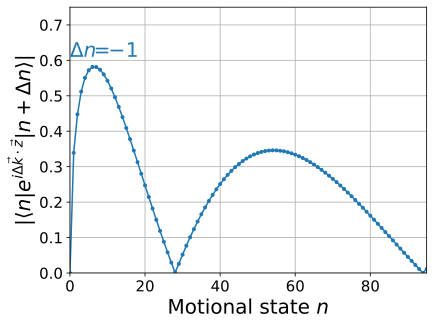
\includegraphics[width=5.5cm]{raman_rabi_1}};
    }
    \visible<6-> {
      \node at (-3, 0) {\includegraphics[width=5.5cm]{raman_rabi_all}};
    }
    \visible<7-> {
      \node[red] at (-3, -3) {3D ground state: $93.5(7)\%$};
    }
    \visible<4-6> {
      \node[align=center] at (3, -2.5) {
        Axial sideband spectrum\\
        \includegraphics[width=6.3cm]{spectrum_az_hot}
      };
    }
    \visible<7-> {
      \node[align=center] at (3, -2.5) {
        Axial sideband spectrum\\
        \includegraphics[width=6.3cm]{spectrum_az}
      };
    }
  \end{tikzpicture}
\end{frame}

\section{Atom-Atom Interaction and Molecule Formation}

\begin{frame}{Outline}
  \tableofcontents[currentsection]
\end{frame}

% So after getting both atom into a single quantum state,
% we can finally study their interaction and make molecules.

% The way we want to make molecule is by optical transfer.
% Essentially drive a transition from the atomic to the molecular state.
% This spare us of a huge FB coil although we are also working on that at the same time

% So we started in atomic state in the potential, here...
% Want to get to here since it's the state with the strongest dipole moment.
% The energy difference is huge and the wavefunction is dissimilar.
% So even though in an ideal world we might be able to do the transfer a single step,
% it's at least technically challenging to pull it off.

% Two steps
% First step (Raman) that replaces the FB association to transfer to a loosely bound state
% Then the same as previous experiement using a STIRAP.
% By splitting the two, we can do the slow inital transfer with a smaller energy difference
% and therefore easier to manage with the laser
% Do the big gap faster
\begin{frame}{Optical Transfer to Molecular State}
  \begin{center}
    \begin{tikzpicture}
      \visible<-2> {
        \shade[ball color=blue!90] (-1, 0) circle (0.45);
        \shade[ball color=orange!90] (-0.6, 0.2) circle (0.3);
        \draw[<->,line width=1] (-1.45, 0.4) -- (-0.65, 0.8);
        \path (-1.05, 0.6) node[rotate=26.565,above=2pt] {$\approx 4a_0$};
        \path (-0.8, 2.4) node[below,align=center] {Binding energy\\$\approx 150 \mathrm{THz}$};
        \path (-0.8, -2) node[below] {\textbf{Molecule}};

        \draw[line width=1] plot[samples=200,domain=-2:2,variable=\x] ({\x + 7}, {(\x)^2 * 0.8 - 1.5});
        \draw[line width=2,orange!90!black]
        plot[samples=200,domain=-2:2,variable=\x] ({\x + 7}, {exp(-(\x)^2 * 1.3) - 0.988});
        \draw[line width=0.8] (7 - 0.8, -0.988) -- (7 + 0.8, -0.988);
        \draw[<->,line width=1] (7 - 1, 0.3) -- (7 + 1, 0.3);
        \path (7, 0.3) node[above] {$\approx 1000a_0$};
        \path (7, -2) node[below] {\textbf{Atoms}};
      }
      \visible<2> {
        \shade[ball color=blue!90] (2.3, -0.1) circle (0.55);
        \shade[ball color=orange!90] (3.1, 0.3) circle (0.4);
        \draw[<->,line width=1] (1.65, 0.4) -- (3.25, 1.2);
        \path (2.45, 0.8) node[rotate=26.565,above=2pt] {$\approx 20a_0$};
        \path (2.7, 2.5) node[below,align=center] {Binding energy\\$\approx 300 \mathrm{MHz}$};
        \path (2.7, -2) node[below,align=center] {\textbf{Weakly-Bound}\\\textbf{Molecule}};
      }
      \visible<3->{
        \begin{scope}[shift={(0, -4)}, scale=0.9]
          \draw[->,line width=1.2] (0, 0) -- (0, 8);
          \node[above,rotate=90] at (0, 4) {Energy};
          \draw[->,line width=1.2] (0, 0) -- (8, 0);
          \node[below] at (4, -0.5) {Internuclear distance};

          \draw[cyan!85!blue] (1.0269 + 0.25, 2.5) -- (7.25, 2.5);
          \draw[cyan!85!blue] (1.0793 + 0.25, -0.4631 + 2.5) -- (4.5 + 0.25, -0.4631 + 2.5);

          \draw[line width=1.1,cyan!85!blue]
          plot[samples=200,domain=1:7,variable=\x]
          ({\x + 0.25}, {6.8*\x^(-3.4)-6.5*\x^(-1.7) + 2.5});
          \node[cyan!85!blue] at (3.75, 1.0) {$a^3\Sigma^+$};

          \draw[line width=1.1,red]
          plot[samples=200,domain=1:7.5,variable=\x]
          ({\x - 0.75}, {9.2*\x^(-2.5)-9.0*\x^(-1.3) + 7.5});
          \node[above right,red] at (0.55, 7.2) {$c^3\Sigma^+$};

          \mytweezer.drawNaAtom(6.55, 2.6, 0.12)
          \mytweezer.drawCsAtom(7.05, 2.6, 0.10)

          \mytweezer.drawNaAtom(4.08, 2.15, 0.12)
          \mytweezer.drawCsAtom(4.25, 2.15, 0.10)

          \draw[black!40,dashed,line width=1] (0.25, 5) -- (7.25, 5);

          \draw[->,green!80!black,line width=1.2] (6.8, 2.7) -- (5.5, 5);
          \draw[->,green!80!black,line width=1.2] (5.45, 5) -- (4.165, 2.25);
        \end{scope}
      }
    \end{tikzpicture}
  \end{center}
\end{frame}

% Raman transfer obviously need some information about the excited state
% So that's what we set out to measure first. (i.e. PA spectroscopy)

% We really have the most textbook system to do this measurement.
% We only have two atoms
% We know the initial state
% We shine some light on it, which might create some excited state molecule that
% falls down to some states that we can't see.
% We know the final state

% Full state info, improve signal-to-noise

% We start with near threshold since the lines are denser/easier to see.
% Single body - flat
% Two body - peaks
% Agreement with the theory/see new lines

% Also found deeper lines afterwards with very similar signal so I'm not showing it here.

% Now we know the excited states.
% After measuring this line, we can use add another beam in order to find
% the ground molecular state.
% With one laser parked on the PA resonance, we can scan the frequency of the other.
% When the difference between the two lasers match ... we can create a EIT and stops the
% PA process ...

% We scanned around the theoritical prediction between 200-300 MHz and indeed found the resonance.
\begin{frame}[t]{\alt<-4>{Photoassociation (PA) Spectroscopy}{Electromagnetically Induced Transparency (EIT) Spectroscopy}}
  \vspace{-0.4cm}
  \begin{center}
    \begin{tikzpicture}
      \begin{scope}[shift={(-4.3, -3.3)}, scale=0.7]
        \draw[->,line width=1.2] (0, 0) -- (0, 8);
        \node[above,rotate=90] at (0, 4) {Energy};
        \draw[->,line width=1.2] (0, 0) -- (8, 0);
        \node[below] at (4, -0.1) {Internuclear distance};

        \draw[cyan!85!blue] (1.0269 + 0.25, 2.5) -- (7.25, 2.5);

        \draw[line width=1.1,cyan!85!blue]
        plot[samples=200,domain=1:7,variable=\x]
        ({\x + 0.25}, {6.8*\x^(-3.4)-6.5*\x^(-1.7) + 2.5});
        \node[cyan!85!blue] at (3.75, 1.0) {$a^3\Sigma^+$};

        \draw[line width=1.1,red]
        plot[samples=200,domain=1:7.5,variable=\x]
        ({\x - 0.75}, {9.2*\x^(-2.5)-9.0*\x^(-1.3) + 7.5});
        \node[above right,red] at (0.55, 7.2) {$c^3\Sigma^+$};

        \draw[red] (1.1102 - 0.75, -0.7720 + 7.5) -- (6 - 0.75, -0.7720 + 7.5);
        \draw[red] (1.1576 - 0.75, -1.0595 + 7.5) -- (4.5 - 0.75, -1.0595 + 7.5);

        \mytweezer.drawNaAtom(6.55, 2.6, 0.12)
        \mytweezer.drawCsAtom(7.05, 2.6, 0.10)

        \draw[->,blue!50!orange,line width=0.8] (6.8, 2.7) -- (4.5 - 0.75, -0.85 + 7.5);

        \only<5->{
          \draw[cyan!85!blue] (1.0793 + 0.25, -0.4631 + 2.5) -- (4.5 + 0.25, -0.4631 + 2.5);
          \draw[cyan!85!blue,<->] (3.5, 2.5) -- ++(0, -0.4631) node[midway, left]
          {\tiny $\delta$};
          \mytweezer.drawNaAtom(4.08, 2.15, 0.12)
          \mytweezer.drawCsAtom(4.25, 2.15, 0.10)
          \draw[->,green!80!black,line width=0.8] (4.165, 2.25) -- (4.45 - 0.75, -0.85 + 7.5);
        }
      \end{scope}
      \visible<2-4>{
        \node[text width=5cm] at (4.2, -1) {
          \begin{block}{Single Atom PA}
            \begin{itemize}
            \item Clean initial state
            \item Narrow excitation laser
            \item Final state detection
            \end{itemize}
          \end{block}
        };
      }
      \visible<3>{
        \node at (3, 3) {\includegraphics[width=8cm]{pa-shallow_1b}};
      }
      \visible<4>{
        \node at (3, 3) {\includegraphics[width=8cm]{pa-shallow}};
      }
      \visible<6>{
        \node at (4, 2.5) {\includegraphics[width=5cm]{eit.png}};
      }
    \end{tikzpicture}
  \end{center}
\end{frame}

% With the states that are important to the transition all mapped out,
% we are ready to drive the ground state Raman transition by detuning the two beams further.
\begin{frame}{Optical Transfer to Weakly-Bound Molecular}
  \begin{center}
    \begin{tikzpicture}
      \visible<-4> {
        \begin{scope}[scale=0.7]
          \draw[->,line width=1.2] (0, 0) -- (0, 8);
          \node[above,rotate=90] at (0, 4) {Energy};
          \draw[->,line width=1.2] (0, 0) -- (8, 0);
          \node[below] at (4, -0.5) {Internuclear distance};

          \draw[cyan!85!blue] (1.0269 + 0.25, 2.5) -- (7.25, 2.5);
          \draw[cyan!85!blue] (1.0793 + 0.25, -0.4631 + 2.5) -- (4.5 + 0.25, -0.4631 + 2.5);

          \draw[line width=1.1,cyan!85!blue]
          plot[samples=200,domain=1:7,variable=\x]
          ({\x + 0.25}, {6.8*\x^(-3.4)-6.5*\x^(-1.7) + 2.5});
          \node[cyan!85!blue] at (3.75, 1.0) {$a^3\Sigma^+$};

          \draw[line width=1.1,red]
          plot[samples=200,domain=1:7.5,variable=\x]
          ({\x - 0.75}, {9.2*\x^(-2.5)-9.0*\x^(-1.3) + 7.5});
          \node[above right,red] at (0.55, 7.2) {$c^3\Sigma^+$};

          \mytweezer.drawNaAtom(6.55, 2.6, 0.12)
          \mytweezer.drawCsAtom(7.05, 2.6, 0.10)

          \mytweezer.drawNaAtom(4.08, 2.15, 0.12)
          \mytweezer.drawCsAtom(4.25, 2.15, 0.10)

          \draw[black!40,dashed,line width=1] (0.25, 5) -- (7.25, 5);

          \draw[->,green!80!black,line width=2] (6.8, 2.7) -- (5.5, 5)
          node[midway, right, align=left] {$\approx1038\mathrm{nm}$\\\ \ \ Tweezer};
          \draw[->,green!80!black,line width=2] (5.45, 5) -- (4.165, 2.25);
        \end{scope}
      }
      \visible<2-> {
        \node at (9, 1.5) {\includegraphics[width=4.5cm]{raman_width}};
        \visible<-4>{
          \draw[->,dashed,cyan,line width=1] (6.8, 2.5) -- (3, 1.5);
        }
      }
      \visible<3-> {
        \node[above, align=center] at (9, 4.7) {But no Rabi oscillation};
      }
      \visible<4-> {
        \node[below, align=center] at (9, 4.4) {$\Gamma_e$ is $\approx50\sim100$x theory value.};
      }
      \visible<5-> {
        \node[align=center] at (2.5, 4.5) {
          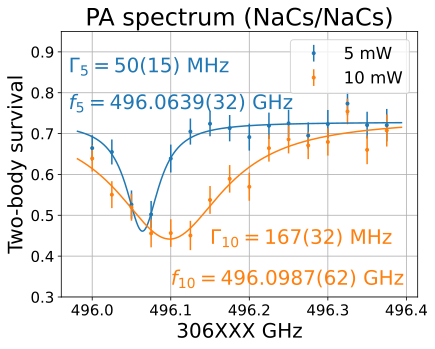
\includegraphics[width=5cm]{../../experiments/pa_201908/imgs/data_20190830_005224_pa_tw_pwr_2b}};
        \node[align=center] at (2.5, 0.45) {
          \includegraphics[width=5cm]{pa_widths}};
      }
    \end{tikzpicture}
  \end{center}
\end{frame}

% Related to/useful for ....
% * Binding energy
% * Molecular potential
% * Feshbach resonance
% * Molecule formation
\begin{frame}{Scattering length $a$}
  \begin{columns}
    \column{4.5cm}
    \begin{itemize}
    \item<2-> Binding energy
    \item<3-> Molecular potential
    \item<4-> Feshbach resonance
    \item<5-> Molecule formation\\
      $\vdots$
    \end{itemize}
    \column{6.5cm}
    \begin{tikzpicture}
      \begin{scope}[scale=0.65]
        \draw[->,line width=1.2] (0, 0) -- (0, 8);
        \node[above,rotate=90] at (0, 4) {Energy};
        \draw[->,line width=1.2] (0, 0) -- (8, 0);
        \node[below] at (4, -0.5) {Internuclear distance};

        \draw[dashed] (1.0269 - 0.25, 2.5) -- (7 - 0.25, 2.5);
        \draw (1.0793 - 0.25, -0.4631 + 2.5) -- (4.5 - 0.25, -0.4631 + 2.5);

        \draw[line width=1.1]
        plot[samples=200,domain=0.8:7,variable=\x]
        ({\x - 0.25}, {6.8*\x^(-3.4)-6.5*\x^(-1.7) + 2.5});

        \mytweezer.drawNaAtom(5.55, 2.7, 0.12)
        \mytweezer.drawCsAtom(6.05, 2.7, 0.10)

        \mytweezer.drawNaAtom(2.08, 2.15, 0.12)
        \mytweezer.drawCsAtom(2.25, 2.15, 0.10)

        \draw[->, cyan!50!blue, line width=0.8] (5.4, 2.7) -- ++(-3.5, 0)
        arc (270:90:0.2) -- ++(2.5, 0);
      \end{scope}
    \end{tikzpicture}
  \end{columns}
\end{frame}

%% When we successfully loaded two atoms in the tweezer,
%% their energy levels will be shifted due to the interaction.
%% This shift depends on the spin state of the atom and we can measure this difference
%% by driving a Raman or microwave transition between HF states.
%% As shown.... by comparing the spectrum with and without another atom...
%% This way of measuring the scattering length is similar to the experiement done
%% in optical lattice on Mott insulator but the anisotropy causes some difference as shown in.

% Interaction shift data
%% One peak on the right, lowering energy -> attractive interaction.
%% Another peak on the left...
%% Significant state mixing due to low axial trapping frequency
%% Theory model
%% 33+22 -> 33+11

\begin{frame}{Interaction shift}
  \vspace{-0.8cm}
  \begin{tikzpicture}
    \draw[white,opacity=0] (-6, -4.5) rectangle (6, 4.5);
    % Raman sequence
    \visible<1>{
      \node at (-2.8, 0.7) {\includegraphics[width=6cm]{shift_raman_1.pdf}};
    }
    \visible<2-3>{
      \node at (-2.8, 0.7) {\includegraphics[width=6cm]{shift_raman.pdf}};
    }
    % Data 1
    \visible<3-6>{\node at (3.2, 0) {\includegraphics[width=5cm]{na2cs4_0.pdf}};}
    \visible<7>{\node at (3.2, 0) {\includegraphics[width=5cm]{na2cs4.pdf}};}
    \visible<8->{\node at (3.2, 0) {\includegraphics[width=5cm]{na2cs3.pdf}};}

    % Equations
    \visible<4-5>{
      \node[below right,align=left] at (-4.9, 3.8)
      {\footnotesize $\displaystyle H=\!\!\sum_{i=x,y,z}(\frac{m_{1}\omega_{1,i}^2x_{1,i}^2}{2}+\frac{p_{1,i}^2}{2m_{1}})\ +\!\sum_{i=x,y,z}(\frac{m_{2}\omega_{2,i}^2x_{2,i}^2}{2}+\frac{p_{2,i}^2}{2m_{2}})+V_{int}(\vec r_1-\vec r_2)$};
      \draw[decoration={brace,mirror,amplitude=10pt},decorate,line width=1]
      (-4.15,2.8) -- node[below=10pt] {\small Na} (-1.15,2.8);
      \draw[decoration={brace,mirror,amplitude=10pt},decorate,line width=1]
      (-0.5,2.8) -- node[below=10pt] {\small Cs} (2.5,2.8);
      \draw[decoration={brace,mirror,amplitude=10pt},decorate,line width=1]
      (3.05,3) -- node[below=10pt] {\small Interaction} (4.55,3);
    }
    \visible<5>{
      \node[above right,align=left] at (-5.8, -2.3)
      {
        \textcolor{blue!60!black}{To center of mass}\\
        \textcolor{blue!60!black}{and relative coordinates}\\
        \\
        {\tiny
          $\begin{aligned}
            M=&\ m_1+m_2&\mu=&\ \frac{m_1m_2}{m_1+m_2}\\
            \Omega_i^2=&\ \frac{m_1\omega_{1,i}^2+m_2\omega_{2,i}^2}{m_1+m_2}&\omega_{R,i}^2=&\ \frac{m_2\omega_{1,i}^2+m_1\omega_{2,i}^2}{m_1+m_2}\\
            X_i=&\ \frac{m_1x_{1,i}+m_2x_{2,i}}{m_1+m_2}&x_{R,i}=&\ x_{1,i}-x_{2,i}\\
            P_i=&\ p_{1,i}+p_{2,i}&p_{R,i}=&\ \frac{m_2p_{1,i}-m_1p_{2,i}}{m_1+m_2}
          \end{aligned}$}};
    }
    \visible<5->{
      \node[above right,align=left] at (-6, -4.5)
      {\footnotesize $\displaystyle H=\!\!\sum_{i=x,y,z}(\frac{M\Omega_{i}^2X_{i}^2}{2}+\frac{P_{i}^2}{2M})\ +\!\sum_{i=x,y,z}(\frac{\mu\omega_{R,i}^2x_{R,i}^2}{2}+\frac{p_{R,i}^2}{2\mu})+V_{int}(\vec r_R)\ +\!\sum_{i=x,y,z}\mu(\omega_{1,i}^2 - \omega_{2,i}^2)X_ix_{R,i}$};
      \draw[decoration={brace,amplitude=10pt},decorate,line width=1]
      (-5.25,-3.5) -- node[above=10pt] {\small Center of mass} (-2.5,-3.5);
      \draw[decoration={brace,amplitude=10pt},decorate,line width=1]
      (-1.9,-3.5) -- node[above=10pt] {\small Relative} (2.4,-3.5);
      \draw[decoration={brace,amplitude=10pt},decorate,line width=1]
      (3,-3.5) -- node[above=10pt] {\small Mixing} (5.9,-3.5);
    }
    \visible<6>{
      \node at (-2.6, 0.5) {\includegraphics[width=6cm]{shift_theory.pdf}};
    }
    \visible<7>{
      \node at (-2.6, 0.5) {\includegraphics[width=6cm]{shift_theory42_32.pdf}};
    }
    \visible<8->{
      \node at (-2.6, 0.5) {\includegraphics[width=6cm]{shift_theory32_31.pdf}};
    }
    \visible<9->{
      \fill[white,opacity=0.95] (-6, -4.5) rectangle (6, 3.5);
      \node[align=center] at (0, 0)
      {Combined with binding energy measurement on Na(2,2) Cs(4,4)\\
        \\
        \begin{tabular}{|c|c|}
          \hline
          Spin state ($F,m_F$)&Scattering length (a.u.)\\\hline
          Na(2,2) Cs(4,4)&30.36\\\hline
          Na(2,2) Cs(3,3)&-693.8\\\hline
          Na(1,1) Cs(3,3)&13.19\\\hline
        \end{tabular}};
    }
    \visible<10->{
      \draw[->, line width=1, color=red!50!black] (0.8, -0.65) -- (-1, -2)
      node[below] {$\sim50$ enhanced coupling to molecular state};
    }
  \end{tikzpicture}
\end{frame}

% Another thing we can measure is the FB resonance
%% Better prediction than before.
\begin{frame}[t]{Na (1, -1) Cs (3, -3) Feshbach resonance}
  \only<1>{
    \begin{center}
      \includegraphics[height=7cm]{chamber1_5.jpg}
    \end{center}
  }
  \only<2->{
    \begin{center}
      \includegraphics[width=10cm]{fb.pdf}\\
      \vspace{0.5cm}
    \end{center}
  }
  \only<3->{
    \begin{center}
      \begin{tabular}{|c|p{1.9cm}|p{1.9cm}|}
        \hline
        &$s$-wave&$p$-wave\\\hline
        Predicted {\tiny (based on interaction shift)\footnote{In collaboration with Bo Gao}}&$663$ G&$799$ G\\\hline
        Measured&$652(3)$ G&$791.2(2)$ G\\\hline
      \end{tabular}
    \end{center}
  }
\end{frame}

\begin{frame}{Summary}
  \begin{itemize}
  \item A single Na and Cs atom prepared in the motional ground state of the same optical tweezer.
  \item Photoassociation and Raman transfer to weakly-bound state.
  \item Characterized Na-Cs scattering and observed first Feshbach resonances.
  \end{itemize}
\end{frame}

\begin{frame}{}
\end{frame}

\begin{frame}{}
\end{frame}

\end{document}
